\documentclass[12pt,a4paper]{article}

\usepackage{geometry}
\usepackage[page,toc]{appendix}

\geometry{a4paper,top=2.5cm,bottom=2.5cm,left=2.5cm,right=2.5cm}
\usepackage[T1]{fontenc}
\usepackage[utf8]{inputenc}
\usepackage[english]{babel}
\usepackage[parfill]{parskip}

\usepackage{caption}
\usepackage{subcaption}
\captionsetup{font=footnotesize}

%\usepackage{xurl}
\usepackage{hyperref}
\usepackage{graphicx}
\usepackage{float}
\usepackage{booktabs}
\usepackage{tabularx}
\usepackage{wrapfig}
\usepackage{listings}
\usepackage[dvipsnames]{xcolor}
\usepackage{javalisting}
\usepackage{ulem}

\usepackage{fancyvrb}

%Setting listing
\definecolor{mygreen}{rgb}{0,0.6,0}
\definecolor{mygray}{rgb}{0.5,0.5,0.5}
\definecolor{mymauve}{rgb}{0.58,0,0.82}

\lstset{
	basicstyle=\footnotesize\sffamily\color{black},
	frame=single,
	numbers=left,
	numbersep=5pt,
	numberstyle=\tiny\color{gray},
	showspaces=false,
	showstringspaces=false,
	tabsize=1,
	literate={\$}{{\textcolor{orange}{\$}}}1,
}

\lstdefinelanguage{Kotlin}{
	comment=[l]{//},
	commentstyle={\color{gray}\ttfamily},
	emph={filter, first, firstOrNull, forEach, lazy, map, mapNotNull, println},
	emphstyle={\color{OrangeRed}},
	identifierstyle=\color{black},
	keywords={!in, !is, abstract, actual, annotation, as, as?, break, by, catch, class, companion, const, constructor, continue, crossinline, data, delegate, do, dynamic, else, enum, expect, external, false, field, file, final, finally, for, fun, get, if, import, in, infix, init, inline, inner, interface, internal, is, lateinit, noinline, null, object, open, operator, out, override, package, param, private, property, protected, public, receiveris, reified, return, return@, sealed, set, setparam, super, suspend, tailrec, this, throw, true, try, typealias, typeof, val, var, vararg, when, where, while},
	keywordstyle={\color{NavyBlue}\bfseries},
	morecomment=[s]{/*}{*/},
	morestring=[b]",
	morestring=[s]{"""*}{*"""},
	ndkeywords={@Deprecated, @JvmField, @JvmName, @JvmOverloads, @JvmStatic, @JvmSynthetic, Array, Byte, Double, Float, Int, Integer, Iterable, Long, Runnable, Short, String, Any, Unit, Nothing, @QActor,
		@QakContext, @HostName, @State, @Initial, @WhenDispatch, @WhenRequest, @WhenReply, @WhenEvent, @EpsilonMove, @WhenTime, state, action, transition},
	ndkeywordstyle={\color{BurntOrange}\bfseries},
	sensitive=true,
	stringstyle={\color{ForestGreen}\ttfamily},
}

\lstdefinelanguage{Go}%
{morekeywords=[1]{package,import,func,type,struct,return,defer,panic,%
		recover,select,var,const,iota,},%
	morekeywords=[2]{string,uint,uint8,uint16,uint32,uint64,int,int8,int16,%
		int32,int64,bool,float32,float64,complex64,complex128,byte,rune,uintptr,%
		error,interface},%
	morekeywords=[3]{map,slice,make,new,nil,len,cap,copy,close,true,false,%
		delete,append,real,imag,complex,chan,},%
	morekeywords=[4]{for,break,continue,range,go,goto,switch,case,fallthrough,if,%
		else,default,},%
	morekeywords=[5]{Println,Printf,Error,Print,},%
	sensitive=true,%
	morecomment=[l]{//},%
	morecomment=[s]{/*}{*/},%
	morestring=[b]',%
	morestring=[b]",%
	morestring=[s]{`}{`},%
}

\definecolor{mygreen}{rgb}{0,0.6,0}
\definecolor{mygray}{rgb}{0.5,0.5,0.5}
\definecolor{mymauve}{rgb}{0.58,0,0.82}

\lstset{ %
	backgroundcolor=\color{white},   % choose the background color
	basicstyle=\footnotesize,        % size of fonts used for the code
	breaklines=true,                 % automatic line breaking only at whitespace
	captionpos=b,                    % sets the caption-position to bottom
	commentstyle=\color{mygreen},    % comment style
	escapeinside={\%*}{*)},          % if you want to add LaTeX within your code
	keywordstyle=\color{blue},       % keyword style
	stringstyle=\color{mymauve},     % string literal style
}


%Commands
\newcommand{\Kotlin}{\texttt{Kotlin} }
\newcommand{\Go}{\texttt{Go} }

%Title
\title{
	\textbf{Coroutine against Goroutine:\\comparison between \textit{Kotlin} and \textit{GoLang} concurrency}\\
	[0.2em]\small Activity Project in \textit{Operating Systems M}
}
\author{Luca Marchegiani}

\begin{document}
	\maketitle
	\tableofcontents
	
	%Body -----------------------------------------------------------------------------------
	\section*{Abstract}

In this paper we are going to make a comparison between \Kotlin and \Go concurrency that is the main focus of the activity project in \textit{Operating Systems M} course of the master degree in \textit{Computer Science Engineering} at the \textit{Alma Mater Studiorum} University of Bologna.

After a description of the concurrency management in these two languages, we will try to go into an experimental comparison using a previously made projects of the author in the courses of \textit{Software System Engineering} and \textit{Mobile Systems M}. 
	\section{Introduction}

\Kotlin is a modern multiplatform programming language developed by \href{https://www.jetbrains.com/}{Jetbrains} that works on JVM such as \href{www.scala-lang.org}{\texttt{Scala}}.
\Kotlin is completely interoperable with \texttt{Java}\footnote{All classes written in \Kotlin are callable from \texttt{Java} code and vice-versa.} and it is \textit{Object-oriented} with strong elements of \href{https://en.wikipedia.org/wiki/Functional_programming}{functional programming} that make it more powerful than his father \texttt{Java}.
As specified in the \href{https://kotlinlang.org/#why-kotlin}{main page} of the official website, \Kotlin has also the advantages to be \textit{concise}, \textit{safe in nullability}, \textit{expressive} \textit{interoperable} and \textit{multiplatform}.

In addition to this, \Kotlin is now the official \texttt{Android} language, and now supports also \href{https://kotlinlang.org/docs/multiplatform.html}{multiplatform} allowing the developer to write \Kotlin code that can be compiled for \href{https://kotlinlang.org/docs/native-overview.html}{native} platform (including \texttt{Android} and \texttt{iOS}), \texttt{JVM} and \texttt{JavaScript}.

\Go is an open source programming language developed and supported by \texttt{Google}.
It's an \textit{imperative} and \textit{object-oriented} language strongly designed for concurrency thanks to its very easy way to launch process.
The idea of this language is to maintain the run-time efficiency of \texttt{C} but with more readability and usability. Differently from \texttt{C}, \Go has \textit{memory safety}, \textit{garbage collection} and \textit{structural typing} as said by \href{https://en.wikipedia.org/wiki/Go_(programming_language)}{Wikipedia}.

\textbf{Both of this language supports \href{https://en.wikipedia.org/wiki/Coroutine}{coroutines}} as concurrent units of execution. \textit{Coroutines} are lightweight processes that can run over multiple OS threads allowing to save on thread management costs.

Coroutines and threads are very similar but the main difference is that the firsts are \textit{non-preemptive} (or \textit{cooperatives}) differently from the seconds that are typically \textit{preemptive} and scheduled by the OS. Indeed, the execution of a coroutine can be suspended and resumed by the developer, calling some operations, and not by the OS.
	\section{Overview of the concurrency in \Kotlin and \Go}

As specified in the introduction, \Kotlin and \Go exposes concurrency thanks to \textbf{coroutines} and other tools that let the developer manage their synchronization.

As we already said, coroutines are lightweight processes for cooperation that executes on OS threads and that can suspend at a certain point and later resumed at the same point but with the possibility to execute on a different thread. The main advantage by using coroutines instead threads is that switching between then does not require any \textit{system call} ensuring lower management costs.
This introduces great advantages especially for \textit{asynchronous} computation.

\subsection{\Kotlin concurrency overview}

We said that \Kotlin is based on the \texttt{JVM} (but can also compile \texttt{JavaScript} or native using \href{https://llvm.org/}{LLVM}) and is interoperable with \texttt{Java}. The main implementation of \Kotlin is done in its compiler: for \Kotlin on \texttt{JVM}, all classes are compiled as normal \texttt{Java} classes. This means that \textbf{\Kotlin can access to all \texttt{threading}} packages exposed by \texttt{Java} (and this is also valid for \texttt{Android}). So, in \Kotlin \textbf{it is possible to use the standard threads} that are provided by \texttt{Java}.

Even if there is the possibility to use the standard \texttt{Java} threads, as anticipated, \Kotlin introduces the new \href{https://github.com/Kotlin/kotlinx.coroutines}{\texttt{kotlinx.coroutines}} library for realizing concurrency by adopting \textit{coroutines}. Coroutines are \textit{instances of suspendable computation} that let the developer to easily write \textbf{asynchronous and non-blocking code} that can run concurrently, without using \textit{callback} or \textit{promises}.
The main mechanism in which \Kotlin coroutines are based is the \textbf{suspending function}: special \Kotlin method that can suspend the execution of the current coroutine without blocking the current thread.

\subsubsection{Realization of coroutines in \Kotlin}

To go into the details of the coroutine in \Kotlin, we have to introduce some basic concepts\footnote{See \href{https://medium.com/mobile-app-development-publication/kotlin-coroutine-scope-context-and-job-made-simple-5adf89fcfe94}{medium.com} for additional details.}:
\begin{itemize}
	\item \href{https://kotlinlang.org/api/kotlinx.coroutines/kotlinx-coroutines-core/kotlinx.coroutines/-job/}{\underline{\textbf{\textcolor{ForestGreen}{Job}}}}:\\
	The object that represents a \textit{background job} of a coroutine. When a coroutine is launched, the \href{https://kotlinlang.org/api/kotlinx.coroutines/kotlinx-coroutines-core/kotlinx.coroutines/launch.html}{\texttt{launch}} method immediately returns the reference to the \texttt{Job} associated to the coroutine. \textbf{A job represents the lifecycle of a coroutine} and can be used to \textit{cancel} its execution. Then, a job can have six possible states, each coded by a combination of the three property of the \texttt{Job} class: \texttt{isActive}, \texttt{isCompleted} and \texttt{isCancelled}.
	This table summarizes the possible states of a \texttt{Job} and the value of the three property for each state:
	\begin{table}[h!]
		\centering
		\begin{tabular}{ccccc}
			\textbf{State} & \textbf{Type} & \textbf{isActive} & \textbf{isCompleted} & \textbf{isCancelled} \\
			\textit{New}        & initial   & \texttt{false} & \texttt{false} & \texttt{false} \\
			\textit{Active}     & initial   & \texttt{true}  & \texttt{false} & \texttt{false} \\
			\textit{Completing} & transient & \texttt{true}  & \texttt{false} & \texttt{false} \\
			\textit{Cancelling} & transient & \texttt{false} & \texttt{false} & \texttt{true}  \\
			\textit{Cancelled}  & final     & \texttt{false} & \texttt{true}  & \texttt{true}  \\
			\textit{Completed}  & final     & \texttt{false} & \texttt{true}  & \texttt{false}
		\end{tabular}
		\caption{States of a \texttt{Job}}
		\label{tab:job_states}
	\end{table}

	\begin{figure}[h!]
		\centering
		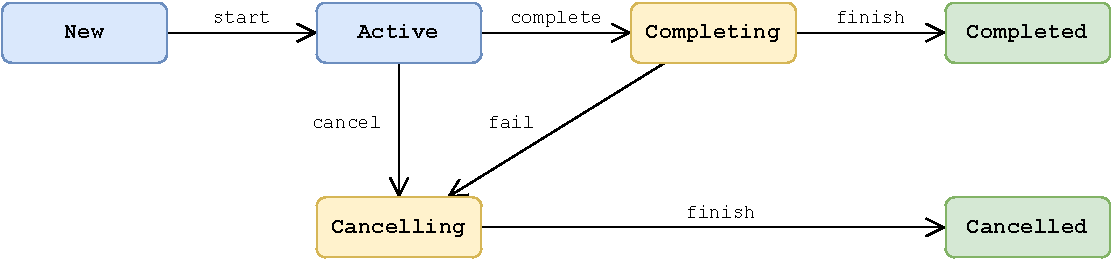
\includegraphics[width=0.9\textwidth]{img/kotlin_coroutines_lifecycle}
		\caption{Lifecycle of \Kotlin coroutine in \texttt{Job}}
		\label{fig::kotlin_coroutines_lifecycle}
	\end{figure}

	The figure \ref{fig::kotlin_coroutines_lifecycle} represents the entire lifecycle of a \texttt{Job}, so it also represents the lifecycle of a \Kotlin coroutine.
	
	\item \href{https://kotlinlang.org/api/kotlinx.coroutines/kotlinx-coroutines-core/kotlinx.coroutines/-coroutine-dispatcher/}{\underline{\textbf{\textcolor{ForestGreen}{CoroutineDispatcher}}}}:\\
	As we already said, in their lifecycle coroutine can run in different threads. For example, suppose to have a coroutine $C_1$ that is started on the thread $T_1$ that executes its code:
	\begin{enumerate}
		\item $C_1$ starts its execution on thread $T_1$;
		\item during its execution, $C_1$ encounter an instruction $I_1$ that suspends it waiting for something;
		\item $C_1$ is suspended by $I_1$ and another coroutine $C_2$ starts to execute on $T_1$;
		\item $C_2$ is executing on $T_1$ while $I_1$ returns resuming $C_1$ from its suspension, but now $T_1$ is not available because it is executing the code of $C_2$;
		\item $C_1$ may execute on another available thread $T_2$ while $C_2$ continue to run in parallel on $T_1$ (if the configuration allows it).
	\end{enumerate}
	\textbf{\texttt{CoroutineDispatcher} is the object that \textit{dispatch} the coroutine in the different available threads}. The \texttt{CoroutineDispatcher} is important because it determines in which thread a couroutine can run: for example, in \texttt{Android} using \href{https://kotlinlang.org/api/kotlinx.coroutines/kotlinx-coroutines-core/kotlinx.coroutines/-dispatchers/-main.html}{Dispatchers.Main} means that the coroutine will be executed confined to the \texttt{Main} thread\footnote{In this case, the coroutine can update the \texttt{UI}. There are also dispatchers for \texttt{JavaFX} or \texttt{Swing} for \texttt{Kotlin JVM} to force coroutines to be executed on the thread that can update the user interface.}.
	
	By default, when a coroutine is created, it is used the \href{https://kotlinlang.org/api/kotlinx.coroutines/kotlinx-coroutines-core/kotlinx.coroutines/-dispatchers/-default.html}{\texttt{Dispatchers.Default}} that uses \textit{worker} threads, a shared pool of threads on \texttt{JVM} in which coroutines can execute in parallel. 
	
	\item \href{https://kotlinlang.org/api/latest/jvm/stdlib/kotlin.coroutines/-coroutine-context/}{\underline{\textbf{\textcolor{ForestGreen}{CoroutineContext}}}}:\\
	Each coroutine in \Kotlin has a \textit{context} that is \textit{immutable}. A context is simply a set of \textit{elements} that realize the concept of \textit{context} in which the coroutine executes.
	The main elements that are present in a context are:
	\begin{itemize}
		\item the \texttt{Job} that represents the coroutine;
		\item the \texttt{CoroutineDispatcher} that dispatches the execution of coroutine over the threads;
		\item the \texttt{CoroutineName} that is the name associated to the coroutine (useful for debugging);
		\item the \texttt{CoroutineExceptionHandler} that is an handler for all the exception thrown during the execution of the coroutine;
		\item the \texttt{ContinuationInterceptor} that allows to define \textit{how} the coroutine should continue after a resume (a sort of \textit{callback} that is invoked on coroutine resume).
	\end{itemize}
	
	Notice that \textbf{\texttt{CoroutineContext} is immutable, but it is possible to add elements using the plus operator} that produces a new context instance.
	
	\item \href{https://kotlinlang.org/api/kotlinx.coroutines/kotlinx-coroutines-core/kotlinx.coroutines/-coroutine-scope/}{\underline{\textbf{\textcolor{ForestGreen}{CoroutineScope}}}}:\\
	Each coroutine in \Kotlin must have a \textit{scope} which delimits the lifetime of the coroutine. The \texttt{CoroutineScope} consists in only one property: \texttt{coroutineContext}, an instance of \texttt{CoroutineContext}.
	In addition to this, the \texttt{CoroutineScope} has also some \href{https://kotlinlang.org/docs/extensions.html}{\textit{extension functions}} such as \href{https://kotlinlang.org/api/kotlinx.coroutines/kotlinx-coroutines-core/kotlinx.coroutines/launch.html}{\texttt{launch}} that is a builder for coroutines.
	
	Then, when \texttt{launch} is invoked using a \texttt{CoroutineScope}, the function launches a new coroutine and its context is \textit{inherited} from those of the scope.
	In this way, all the elements of the parents and its cancellation are propagated to the child; then, if a scope is cancelled, all the coroutine launched starting from it will be cancelled.
\end{itemize}

\begin{center}
	In \Kotlin \textbf{the concept of \textit{coroutine} can be summarized by the formula}:\\
		\textit{Coroutine} $=$ \texttt{CoroutineContext} $+$ \texttt{Job}
\end{center}

In order to launch a coroutine, the developer has to:
\begin{enumerate}
	\item \underline{create an instance of \texttt{CoroutineScope}}, for example using the \href{https://kotlinlang.org/api/kotlinx.coroutines/kotlinx-coroutines-core/kotlinx.coroutines/run-blocking.html}{\texttt{runBlocking}} scope builder;
	
	\item \underline{call a coroutine builder starting from the created scope}, such as \texttt{launch}, that returns the \texttt{Job} associated to the coroutine.
\end{enumerate}

Here is the example of the creation of a simple coroutine taken from the official documentation on \href{https://kotlinlang.org/docs/coroutines-basics.html#your-first-coroutine}{kotlinlang.org}:
\begin{lstlisting}[language=kotlin]
	fun main() = runBlocking { // this: CoroutineScope
		launch { // launch a new coroutine and continue
			delay(1000L) // non-blocking delay for 1 second (default time unit is ms)
			println("World!") // print after delay
		}
		println("Hello") // main coroutine continues while a previous one is delayed
	}
\end{lstlisting}

that produces this result on the console:
\begin{lstlisting}[numbers=none]
	Hello
	World!
\end{lstlisting}

To fully understand this snippet, the reader should know \href{https://kotlinlang.org/docs/lambdas.html#higher-order-functions}{\textit{higher-order functions}} and \href{https://kotlinlang.org/docs/lambdas.html#function-types}{\textit{receivers}} which are concepts that came from \textit{functional programming} available in \Kotlin.

\subsubsection{Synchronization between coroutines in \Kotlin}

We highlight that \textbf{coroutines in \Kotlin can use shared memory or \textit{messages}} to synchronize themselves. In particular:
\begin{itemize}
	\item \underline{The package \href{https://kotlinlang.org/api/kotlinx.coroutines/kotlinx-coroutines-core/kotlinx.coroutines.sync/}{\texttt{kotlinx.coroutines.sync}}} exposes classical tools for synchronization in a shared memory environment (\textit{mutex} and \textit{semaphore}).
	
	Notice that this type of synchronization is very basic if compared with the standard \texttt{Java} tools for concurrency such as \texttt{Lock} and \texttt{Condition}; at this moment, \Kotlin does not define any mechanism similar to \texttt{Java} condition, but however it's simple to implement it (for example, we have an implementation made by the author called \href{https://github.com/LM-96/KBomber/blob/main/kbomberx-concurrency/src/main/kotlin/kbomberx/concurrency/sync/CoroutineCondition.kt}{\texttt{CoroutineCondition}} that uses the \href{https://kotlinlang.org/api/latest/jvm/stdlib/kotlin.coroutines/-continuation/}{\texttt{Continuation}} object of a coroutine).
	
	\item \underline{The package \href{https://kotlinlang.org/api/kotlinx.coroutines/kotlinx-coroutines-core/kotlinx.coroutines.channels/}{\texttt{kotlinx.coroutines.channels}}} exposes classical tools for synchronization by exchanging messages in no shared memory environment (\textit{channels}).
	The main entity of this package is \href{https://kotlinlang.org/docs/channels.html}{\texttt{Channel}}, that is very similar to \href{https://docs.oracle.com/en/java/javase/18/docs/api/java.base/java/util/concurrent/BlockingQueue.html}{\texttt{BlockingQueue}} but with suspending operations instead of the \texttt{Java} blocking methods.
	
	Two coroutines can use a channel in order to transfer a single value that came from the \textit{producer} (the coroutine that invoke the \texttt{send} operation) and goes to the \textit{consumer} (the coroutine that invoke the \texttt{receive} operation); in \Kotlin channels are \textbf{bidirectional} and \textbf{symmetric} (one-to-one).
	
	\textbf{The semantic of \textit{send/receive} operations depends on the nature of the channel} that is determinated by its capacity, but the communication can be \textbf{synchronous} or \textbf{asynchronous} with also some little variations of these (for example, \textbf{rendez-vous}).
	
	\item \underline{The package \href{https://kotlinlang.org/api/kotlinx.coroutines/kotlinx-coroutines-core/kotlinx.coroutines.flow/}{\texttt{kotlinx.coroutines.flow}}} exposes the tools for using \href{https://kotlinlang.org/docs/flow.html}{\textit{flows}} that are defined by the documentation as \href{https://kotlinlang.org/api/kotlinx.coroutines/kotlinx-coroutines-core/kotlinx.coroutines.flow/L}{\textit{asynchronous cold stream of elements}} that can safely be used to synchronize multiple coroutine at the same time.
	
	Flow can be more formally defined as \textbf{mono-directional, one-to-many and asynchronous} channels with the possibility to be \textbf{buffered} for replay strategies. In the latest versions of \Kotlin, flows replaced \href{https://kotlinlang.org/api/kotlinx.coroutines/kotlinx-coroutines-core/kotlinx.coroutines.channels/-broadcast-channel/}{\texttt{BroadcastChannel}}.
\end{itemize}


	\section{Performance test}

\subsection{Parallel matrix multiplication algorithms}

We will use the matrix multiplication as algorithm to test the performance of \Kotlin and \Go coroutine implementations. There will be three different versions of the algorithm:

\begin{itemize}
	\item \textbf{FAN}:\\
	Uses 2 channels: one to distribute the cells to be computed (\texttt{taskChannel}), the other to collect the partial results (\texttt{resultChannel}); thanks to the \texttt{fan}, all the workers wait on the same channel and send their result on the other. A coordinator is in charge to open the channels, launch the workers, distribute the work, collect the results and finally close the channels, automatically notifying the end of the computation.
	
	\item \textbf{COORDINATOR}:\\
	Requires a coordinator \textit{server} like the previous, but a greater amount of channels: one channel shared  by the workers to notify their availability (\texttt{requestWorkChannel}), one channel the workers can use to notify their termination (\texttt{ackChannel}), one channel to send the partial results (\texttt{resultChannel}), and one channel for each worker the coordinator uses to send the cell to be computed (\texttt{workerChannels[]}). 
	
	The matrices are still on the shared memory and their reference is passed to the workers. The coordinator has to listen both of the \texttt{requestChannel} and the 	\texttt{resultChannel} to react to the availability of a worker or to the computation of a partial result: when all the cells are computed, the coordinator notifies each worker channel, then wait for their termination and returns the final result.
	
	\item \textbf{PURE}\\
	This algorithm is the same of the previous, but the matrices are not in the shared memory anymore, so the coordinator send the row and the column the worker has to use to produce the result for the requested cell.
	
	This is a pure implementation of a message-passing algorithm, without any shared memory but only using channels and messages.
\end{itemize}

\begin{center}
	\begin{tabular}{|>{\raggedright\arraybackslash}p{4cm}|>{\raggedright\arraybackslash}p{4cm}|>{\raggedright\arraybackslash}p{4cm}|}
		\hline
		\textbf{Algorithm} & \textbf{Shared Memory Usage} & \textbf{Number of Channels} \\
		\hline
		\textbf{FAN} & Input Matrices & 2 \\
		\hline
		\textbf{COORDINATOR} & Input Matrices & 3 + $N_{WORKERS}$ \\
		\hline
		\textbf{PURE} & None & 3 + $N_{WORKERS}$ \\
		\hline
	\end{tabular}
\end{center}

While \Kotlin offers a solid \textit{object-oriented} paradigm, \Go has only a minimal support for it: while for the first language we have one interface in its file and the implementation in their own files, all the \Go code is enclosed in a single file following the language's conventions:

\begin{center}
	\begin{tabular}{|>{\raggedright\arraybackslash}p{3cm}|>{\raggedright\arraybackslash}p{9cm}|}
		\hline
		\textbf{Language} & \textbf{Implementations} \\
		\hline
		\Kotlin & 
		\begin{tabular}[t]{@{}l@{}}
			\href{https://github.com/LM-96/Activity-Project-Operating-Systems-M-/blob/main/code/kotlin/unibo.apos.examples/src/main/kotlin/unibo/apos/matrix/product/MatrixProduct.kt}{\texttt{MatrixProduct.kt}} \\
			\href{https://github.com/LM-96/Activity-Project-Operating-Systems-M-/blob/main/code/kotlin/unibo.apos.examples/src/main/kotlin/unibo/apos/matrix/product/impl/FanChanneledMatrixProductImpl.kt}{\texttt{FanChanneledMatrixProductImpl.kt}} \\
			\href{https://github.com/LM-96/Activity-Project-Operating-Systems-M-/blob/main/code/kotlin/unibo.apos.examples/src/main/kotlin/unibo/apos/matrix/product/impl/CoordinatorChanneledMatrixProductImpl.kt}{\texttt{CoordinatorChanneledMatrixProductImpl.kt}} \\
			\href{https://github.com/LM-96/Activity-Project-Operating-Systems-M-/blob/main/code/kotlin/unibo.apos.examples/src/main/kotlin/unibo/apos/matrix/product/impl/PureChanneledMatrixProductImpl.kt}{\texttt{PureChanneledMatrixProductImpl.kt}} \\
		\end{tabular} \\
		\hline
		\Go & 
		\href{https://github.com/LM-96/Activity-Project-Operating-Systems-M-/blob/main/code/go/matrix/matrix.go}{\texttt{matrix.go}} \\
		\hline
	\end{tabular}
\end{center}

\subsection{Main and launchers for performance analysis}

In order to use the algorithm that have just been presented, we need two main application:
\begin{center}
	\begin{tabular}{|>{\raggedright\arraybackslash}p{3cm}|>{\raggedright\arraybackslash}p{9cm}|}
		\hline
		\textbf{Language} & \textbf{Implementations} \\
		\hline
		\Kotlin & 
		\begin{tabular}[t]{@{}l@{}}
			\href{https://github.com/LM-96/Activity-Project-Operating-Systems-M-/blob/main/code/kotlin/unibo.apos.examples/src/main/kotlin/unibo/apos/KAposMatrixApp.kt}{\texttt{KAposMatrixApp.kt}} \\
		\end{tabular} \\
		\hline
		\Go & 
		\href{https://github.com/LM-96/Activity-Project-Operating-Systems-M-/blob/main/code/go/main.go}{\texttt{main.go}} \\
		\hline
	\end{tabular}
\end{center}

Both of the \texttt{main} functions, accept that series of parameters in order to \textbf{perform the computation of the product of two matrices with the specified size, using the given number of coroutines}.
In addition, the programs have been implemented with the possibility to store the results in a \texttt{csv}, specifying a file to go in append mode.

Notice that:
\begin{itemize}
	\item the\uline{ \Kotlin} application must be \uline{built using \href{https://gradle.org/}{\texttt{Gradle}}}, for example via the task \texttt{distZip} that creates a convenient launcher to execute the jar
	\item  the \uline{\Go} application has to be \uline{compiled using \href{https://go.dev/doc/tutorial/compile-install}{\texttt{go build}}}
\end{itemize}

Once the executable are created, they can be invoked using the arguments specified in the following table:

\begin{center}
	\begin{tabular}{|>{\raggedright\arraybackslash}p{3cm}|>{\raggedright\arraybackslash}p{3cm}|>{\raggedright\arraybackslash}p{7cm}|}
		\hline
		\textbf{Option} & \textbf{Default Value} & \textbf{Description} \\
		\hline
		\texttt{-s, --size} & 3 & Size of the matrices (NxN) \\
		\hline
		\texttt{-c, --coroutines} & 4 & Number of coroutines to use \\
		\hline
		\texttt{-o, --output} & \texttt{false} & Store results in CSV file \\
		\hline
		\texttt{-f, --file} & \texttt{null} & CSV filename for storing results \\
		\hline
		\texttt{-r, --repeat} & 1 & Number of times to repeat the calculation \\
		\hline
		\texttt{-l, --log} & false & Enable detailed logging \\
		\hline
		\texttt{-m, --mode} & \texttt{COORDINATOR} & Concurrency mode: \texttt{COORDINATOR}, \texttt{FAN}, or \texttt{PURE} \\
		\hline
	\end{tabular}
\end{center}

\textbf{The argument \texttt{-r} allows to repeat the multiplication for the specified number of times with the given parameters}: each run is then associated to the same \textbf{workspace}.
A workspace is \uline{a set of execution with the same parameters} and it's used in order to perform average logic and enhance the precision of the analysis.

To easily produce the executables and launch them at once with suitable sets of values for the matrix size and the workers, a convenient launcher for \texttt{Linux} has been developed at \href{https://github.com/LM-96/Activity-Project-Operating-Systems-M-/blob/main/code/launcher.sh}{\texttt{launcher.sh}}.

That launcher executes two kind of analysys:

\begin{itemize}
	\item \textbf{FIXED SIZE}\\
	The \uline{size of the matrices is fixed} while \uline{the number of the workers is increased} execution by execution.
	
	\item \textbf{FIXED WORKER}\\
	The \uline{number of the workers is fixed} but \uline{the size of the matrix varies} execution by execution.
\end{itemize}

Each set of $(size, workers)$ is executed for 10 times. This way, then the \texttt{csv} is produced, just the average of the execution times of the repetitions of the same set will be considered.

\subsection{Native compilation for \Kotlin}

\subsubsection{\Kotlin Native}

Kotlin supports \href{https://kotlinlang.org/docs/native-overview.html}{\textbf{native compilation}} realized from the same \texttt{Jetbrains} by involving \href{https://llvm.org/}{LLVM}.

We want to add also \texttt{Kotlin Native} in the comparison to analyze the difference between \texttt{Kotlin JVM} and \Go.

Notice that when \Kotlin is configured to work in the native mode (see \href{https://github.com/LM-96/Activity-Project-Operating-Systems-M-/blob/main/code/kotlin-native/build.gradle.kts}{\texttt{build.gradle.kts}}), the set of usable library is reduced and the \textbf{Java} standard libraries are not supported anymore (even the \texttt{Java IO/NIO}). For this reason, some modifications to the existing \Kotlin code were needed: you can find here the \href{https://github.com/LM-96/Activity-Project-Operating-Systems-M-/tree/main/code/kotlin-native}{\texttt{kotlin-native}} project with the right configuration and a thinner code that allows the compilation.

A convenient launcher as also be developed to launch the native compilation and the execution with the same parameters of the launcher shown in the paragraph above: \href{https://github.com/LM-96/Activity-Project-Operating-Systems-M-/blob/main/code/launcher_ktntv.sh}{\texttt{launcher\_ktntv.sh}}

\subsubsection{\Kotlin compiled via \texttt{GraalVM}}

Java itself supports native compilation thanks to an external and advanced \texttt{JVM} with innovative technologies that supports a process called \href{https://www.graalvm.org/latest/reference-manual/native-image/}{\textit{ahead-of-time Native Image compilation}}.

We will not go deep into the details of this project, but we are going to use it to test this other way to compile native \Kotlin code. Notice that, differently from the previous solution, this one is not developed from \texttt{Jetbrains}, but from an external community of developers. Indeed, \texttt{GraalVM} was initially developed for \texttt{Java} but, since \Kotlin compiles itself \texttt{Java}, it is also compatible without problems.

The configuration of \texttt{GraalVM}'s compilation does not involve complex processes than modifying the \href{https://github.com/LM-96/Activity-Project-Operating-Systems-M-/blob/main/code/kotlin/unibo.apos.examples/build.gradle}{\texttt{build.gradle}} with the proper plugin conveniently configured.

The setup is carefully explained at \href{https://graalvm.github.io/native-build-tools/latest/gradle-plugin.html}{this page} but, as done for the others, we developed a launcher also for the \texttt{GraalVM} version at \href{https://github.com/LM-96/Activity-Project-Operating-Systems-M-/blob/main/code/launcher_graal.sh}{\texttt{launcher\_graal.sh}}.

\subsection{Overview of the considered versions and plotting}

Based on what has been presented, the following table summarizes all the algorithms and the version of the languages we are going to use to perform the analysis:

\begin{center}
	\begin{tabular}{|>{\raggedright\arraybackslash}p{3cm}|>{\raggedright\arraybackslash}p{4cm}|>{\raggedright\arraybackslash}p{3cm}|>{\raggedright\arraybackslash}p{3cm}|}
		\hline
		\textbf{} & \textbf{COORDINATOR} & \textbf{FAN} & \textbf{PURE} \\
		\hline
		\textbf{Kotlin} & \texttt{kt\_coordinator} & \texttt{kt\_fan} & \texttt{kt\_pure} \\
		\hline
		\textbf{Kotlin Native} & \texttt{kt\_ntv\_coordinator} & \texttt{kt\_ntv\_fan} & \texttt{kt\_ntv\_pure} \\
		\hline
		\textbf{Kotlin Graal} & \texttt{kt\_graal\_coordinator} & \texttt{kt\_graal\_fan} & \texttt{kt\_graal\_pure} \\
		\hline
		\textbf{Go} & \texttt{go\_coordinator} & \texttt{go\_fan} & \texttt{go\_pure} \\
		\hline
	\end{tabular}
\end{center}

The results of the executions will be placed into proper csv:
\begin{itemize}
		\item \href{https://github.com/LM-96/Activity-Project-Operating-Systems-M-/blob/main/code/benchmark_results/fixed_size_sel.csv}{\texttt{fixed\_size\_sel.csv}} for the results of the \textit{fixed size} analysis
		
		\item 
		\href{https://github.com/LM-96/Activity-Project-Operating-Systems-M-/blob/main/code/benchmark_results/fixed_workers_sel.csv}{\texttt{fixed\_workers\_sel.csv}} for the results of the \textit{fixed workers} analysis
\end{itemize}

Another component \href{https://github.com/LM-96/Activity-Project-Operating-Systems-M-/tree/main/code/server}{\texttt{server}} has been developed in order to accept the \texttt{csv} files and produce the graph we are going to show.

Again, we developed a script to easily call the server to produce the graphs: \href{https://github.com/LM-96/Activity-Project-Operating-Systems-M-/blob/main/code/graphs.sh}{\texttt{graphs.sh}}

\subsection{All-in-one graphs}

\begin{figure}[H]
	\centering
	\begin{minipage}{0.7\textwidth}
		\centering
		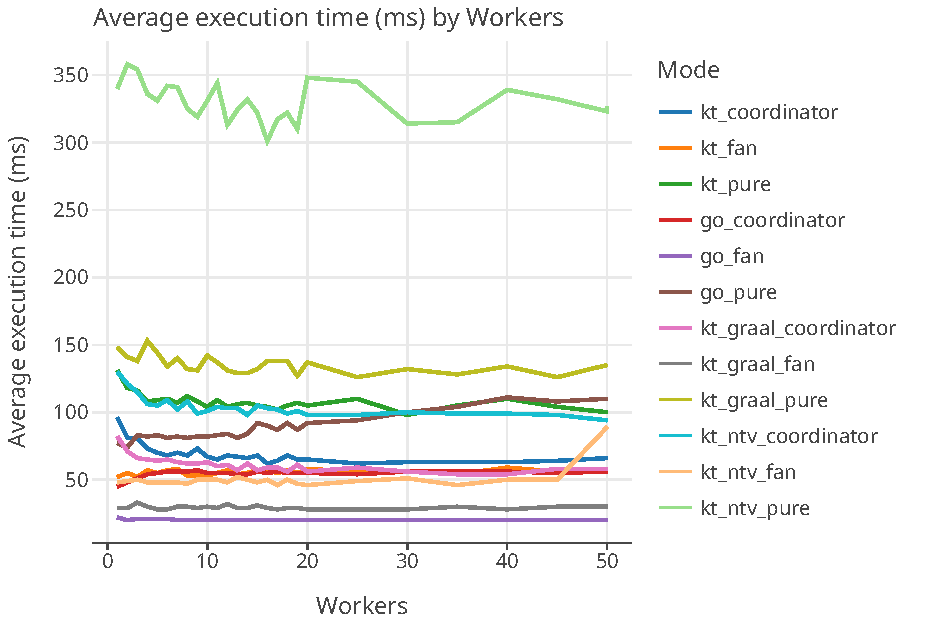
\includegraphics[width=\textwidth]{img/graphs/fixed_size_all}
		\caption{Fixed Size Analysis}
	\end{minipage}\hfill
	\begin{minipage}{0.25\textwidth}
		The graph clearly shows a huge variety of performance between the different variants.  We can see that \Go \texttt{FAN} has the best performance, followed by \Kotlin Graal at the same variant.
		Without any doubt, the worse is \Kotlin Native in pure mode, meaning that pure message-passing communication could not be optimized in the native compiled sources.
	\end{minipage}
\end{figure}

\begin{figure}[H]
	\centering
	\begin{minipage}{0.7\textwidth}
		\centering
		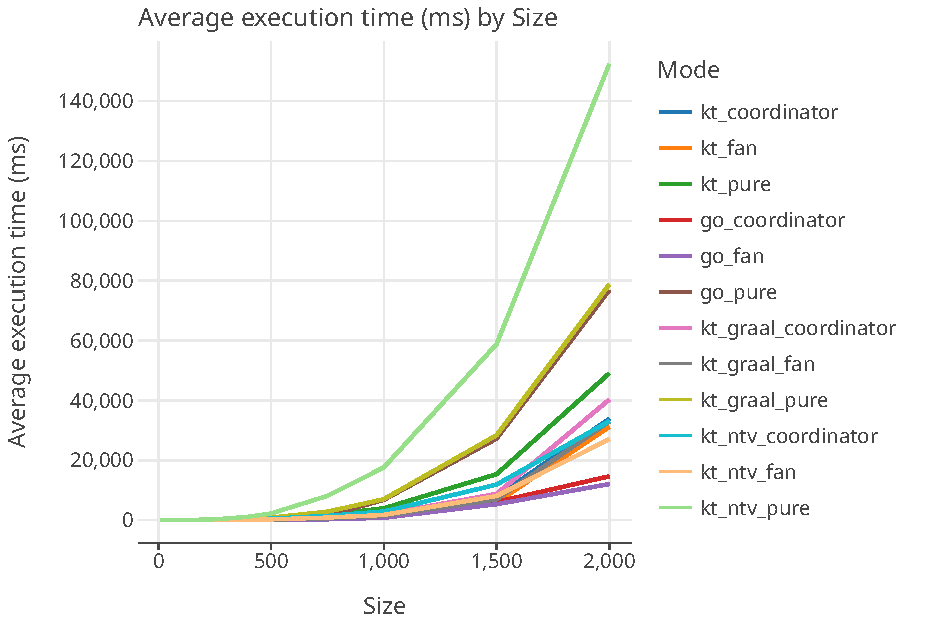
\includegraphics[width=\textwidth]{img/graphs/fixed_workers_all}
		\caption{Fixed Worker Analysis}
	\end{minipage}\hfill
	\begin{minipage}{0.25\textwidth}
		Also this graph seems to confirm the impressions above, with \Kotlin Native having the worst performance. Anyway, \Kotlin Native in the \texttt{FAN} mode performs slightly well, but \Go confirms to be less time-consuming both in the \texttt{FAN} and \texttt{COORDINATOR} modes. Anyway, the \texttt{PURE} modes have the worst times while the \texttt{FAN} have the bests.
	\end{minipage}
\end{figure}

\subsection{Graphs by modes}

\subsubsection{Fixed size}

\begin{figure}[H]
	\centering
	\begin{minipage}{0.7\textwidth}
		\centering
		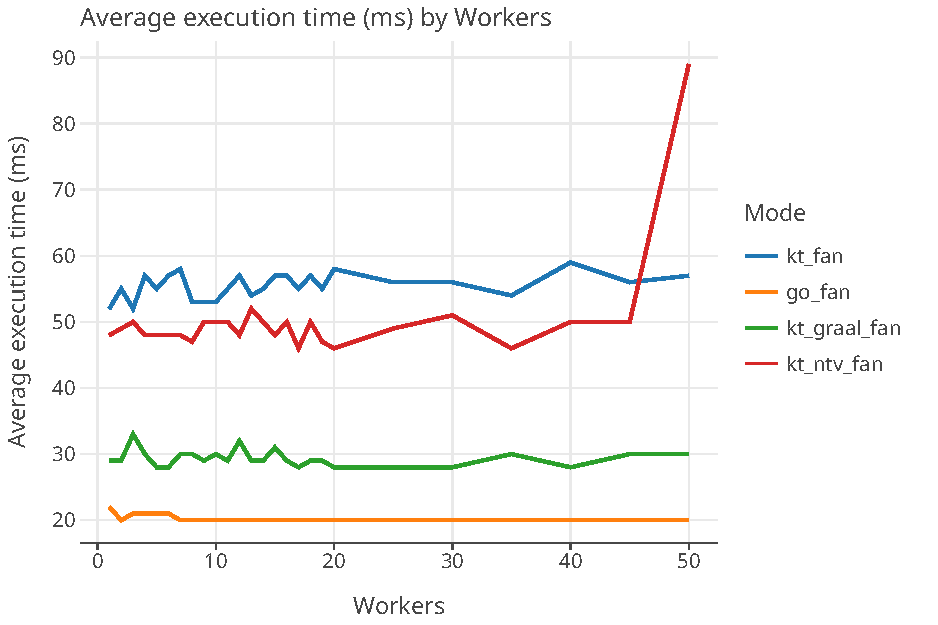
\includegraphics[width=\textwidth]{img/graphs/fixed_size_fan}
		\caption{Fixed Size Analysis \texttt{FAN}}
	\end{minipage}\hfill
	\begin{minipage}{0.25\textwidth}
		\Go and \Kotlin \texttt{Graal} still are the bests while \Kotlin Native initially seems to be winning on \texttt{JVM}, but it definitively looses with a huge number of workers. In addition, \Go seems to resist really well to the increase of the workers, keeping the execution time almost constant and demonstrating a huge ability to handle a significant amount of concurrent units.
	\end{minipage}
\end{figure}

\begin{figure}[H]
	\centering
	\begin{minipage}{0.7\textwidth}
		\centering
		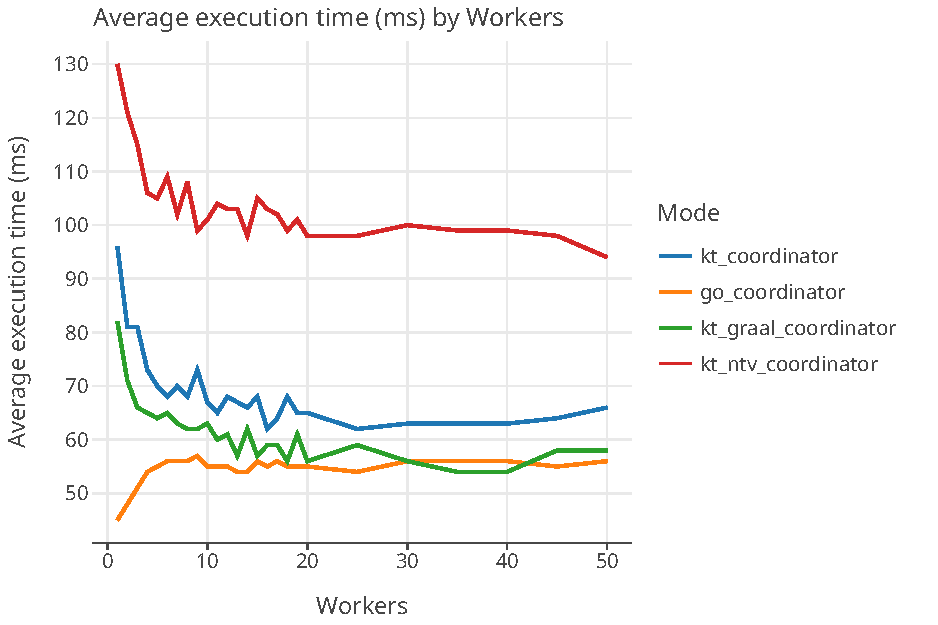
\includegraphics[width=\textwidth]{img/graphs/fixed_size_coordinator}
		\caption{Fixed Size Analysis  \texttt{COORDINATOR}}
	\end{minipage}\hfill
	\begin{minipage}{0.25\textwidth}
		\Go still confirms as the one that takes less time while \Kotlin Native keeps being the worst.
		\texttt{GraalVM} demonstrate to be a competitive solution.
	\end{minipage}
\end{figure}

\begin{figure}[H]
	\centering
	\begin{minipage}{0.7\textwidth}
		\centering
		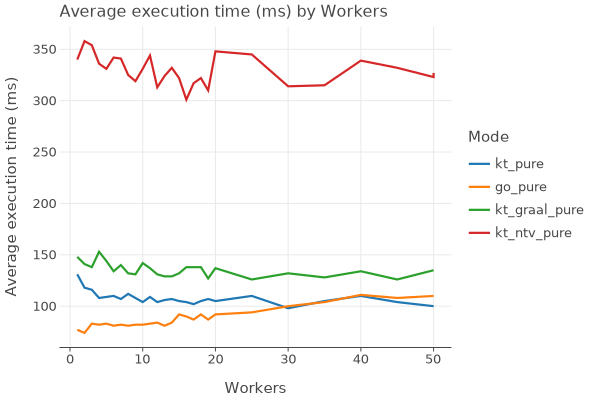
\includegraphics[width=\textwidth]{img/graphs/fixed_size_pure}
		\caption{Fixed Size Analysis \texttt{PURE}}
	\end{minipage}\hfill
	\begin{minipage}{0.25\textwidth}
		We can see that \Kotlin native incredibly suffers with the pure variant, showing that the native compilation is not optimized with channels communication. Instead, the \texttt{JVM} seems to have a good optimization of the message-passing technology. 
	\end{minipage}
\end{figure}

\subsubsection{Fixed workers}

\begin{figure}[H]
	\centering
	\begin{minipage}{0.7\textwidth}
		\centering
		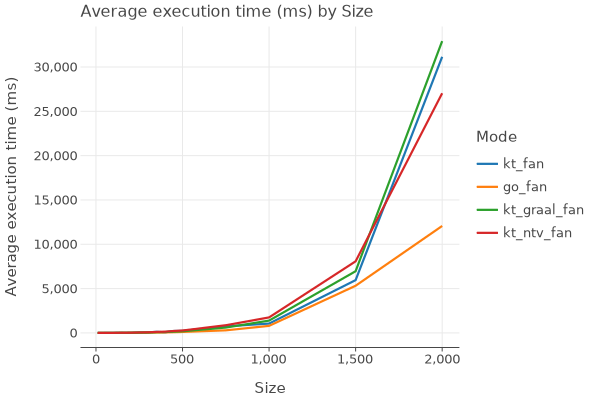
\includegraphics[width=\textwidth]{img/graphs/fixed_workers_fan}
		\caption{Fixed Workers Analysis \texttt{FAN}}
	\end{minipage}\hfill
	\begin{minipage}{0.25\textwidth}
		\Go keeps to be the one with the minimum elapsed times, while \texttt{Graal} shows some worsening especially with the increasing of the size.
	\end{minipage}
\end{figure}

\begin{figure}[H]
	\centering
	\begin{minipage}{0.7\textwidth}
		\centering
		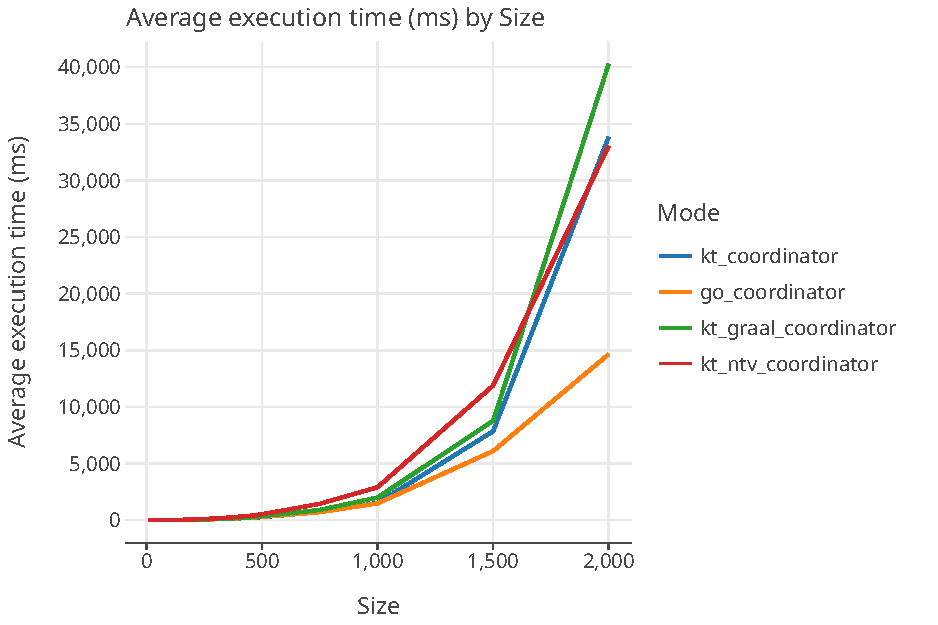
\includegraphics[width=\textwidth]{img/graphs/fixed_workers_coordinator}
		\caption{Fixed Workers Analysis  \texttt{COORDINATOR}}
	\end{minipage}\hfill
	\begin{minipage}{0.25\textwidth}
		The graphs is really similar to the previous one, with \Go as the best, \texttt{Graal} that suffers when the size increases while \Kotlin Native seems to recover some points at the end.
	\end{minipage}
\end{figure}

\begin{figure}[H]
	\centering
	\begin{minipage}{0.7\textwidth}
		\centering
		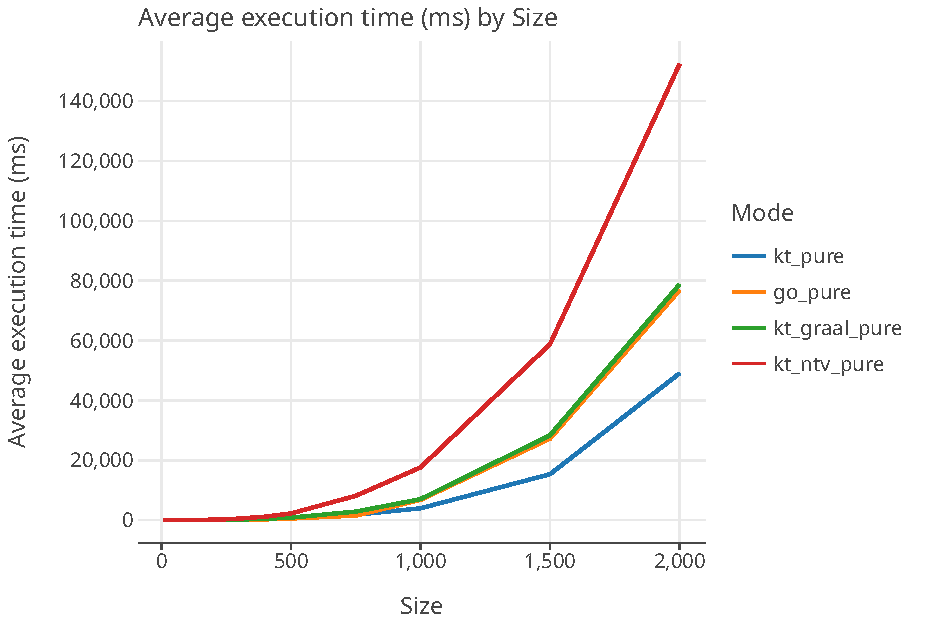
\includegraphics[width=\textwidth]{img/graphs/fixed_workers_pure}
		\caption{Fixed Workers Analysis \texttt{PURE}}
	\end{minipage}\hfill
	\begin{minipage}{0.25\textwidth}
		This graph shows some improvements for the \texttt{JVM} while \texttt{Graal} and \Go behave really similar. \Kotlin Native keeps to be the worst.
	\end{minipage}
\end{figure}

\subsection{The behavior of the \texttt{JVM} with multiple executions}

One of the reason why the coroutines have success on the \texttt{JVM}, is because they let to pay the cost of the Thread's creation only once. Then, since the Threads remains active and the coroutines are scheduled across them, the \texttt{JVM} does not have to loose time managin activation or de-activation of the them, saving lots of time.

This can be seen zooming into one of the \texttt{csv}, focusing on \Kotlin \texttt{JVM}:

\begin{lstlisting}
	workspaceId,size,coroutine,mode,timeMillis
	612f53a2-3b8b-4e39-84ee-0ee64bf1c89e,250,1,kt_coordinator,272
	612f53a2-3b8b-4e39-84ee-0ee64bf1c89e,250,1,kt_coordinator,102
	612f53a2-3b8b-4e39-84ee-0ee64bf1c89e,250,1,kt_coordinator,96
	612f53a2-3b8b-4e39-84ee-0ee64bf1c89e,250,1,kt_coordinator,89
	612f53a2-3b8b-4e39-84ee-0ee64bf1c89e,250,1,kt_coordinator,86
	612f53a2-3b8b-4e39-84ee-0ee64bf1c89e,250,1,kt_coordinator,80
	612f53a2-3b8b-4e39-84ee-0ee64bf1c89e,250,1,kt_coordinator,61
	612f53a2-3b8b-4e39-84ee-0ee64bf1c89e,250,1,kt_coordinator,61
	612f53a2-3b8b-4e39-84ee-0ee64bf1c89e,250,1,kt_coordinator,61
	612f53a2-3b8b-4e39-84ee-0ee64bf1c89e,250,1,kt_coordinator,61
\end{lstlisting}

\textbf{As we can see, the time of the first execution is almost 4.45 times the last one}. This is not happening to the compiled versions of \Go and \Kotlin Native, while the \texttt{Graal} show a significant improvement:

\begin{lstlisting}
	workspaceId,size,coroutine,mode,timeMillis
	324fbed9-a3a9-43af-b9be-add5ae409379,250,1,go_coordinator,48
	324fbed9-a3a9-43af-b9be-add5ae409379,250,1,go_coordinator,42
	324fbed9-a3a9-43af-b9be-add5ae409379,250,1,go_coordinator,48
	324fbed9-a3a9-43af-b9be-add5ae409379,250,1,go_coordinator,49
	324fbed9-a3a9-43af-b9be-add5ae409379,250,1,go_coordinator,47
	324fbed9-a3a9-43af-b9be-add5ae409379,250,1,go_coordinator,45
	324fbed9-a3a9-43af-b9be-add5ae409379,250,1,go_coordinator,44
	324fbed9-a3a9-43af-b9be-add5ae409379,250,1,go_coordinator,49
	324fbed9-a3a9-43af-b9be-add5ae409379,250,1,go_coordinator,42
	324fbed9-a3a9-43af-b9be-add5ae409379,250,1,go_coordinator,42
	ce8edcc7-1d94-427b-9d55-af4dbdd1d515,250,1,kt_graal_coordinator,132
	ce8edcc7-1d94-427b-9d55-af4dbdd1d515,250,1,kt_graal_coordinator,74
	ce8edcc7-1d94-427b-9d55-af4dbdd1d515,250,1,kt_graal_coordinator,76
	ce8edcc7-1d94-427b-9d55-af4dbdd1d515,250,1,kt_graal_coordinator,76
	ce8edcc7-1d94-427b-9d55-af4dbdd1d515,250,1,kt_graal_coordinator,76
	ce8edcc7-1d94-427b-9d55-af4dbdd1d515,250,1,kt_graal_coordinator,81
	ce8edcc7-1d94-427b-9d55-af4dbdd1d515,250,1,kt_graal_coordinator,76
	ce8edcc7-1d94-427b-9d55-af4dbdd1d515,250,1,kt_graal_coordinator,76
	ce8edcc7-1d94-427b-9d55-af4dbdd1d515,250,1,kt_graal_coordinator,81
	ce8edcc7-1d94-427b-9d55-af4dbdd1d515,250,1,kt_graal_coordinator,77
	727f-3326-faf8-efb0,250,1,kt_ntv_coordinator,132
	727f-3326-faf8-efb0,250,1,kt_ntv_coordinator,130
	727f-3326-faf8-efb0,250,1,kt_ntv_coordinator,169
	727f-3326-faf8-efb0,250,1,kt_ntv_coordinator,123
	727f-3326-faf8-efb0,250,1,kt_ntv_coordinator,124
	727f-3326-faf8-efb0,250,1,kt_ntv_coordinator,125
	727f-3326-faf8-efb0,250,1,kt_ntv_coordinator,126
	727f-3326-faf8-efb0,250,1,kt_ntv_coordinator,128
	727f-3326-faf8-efb0,250,1,kt_ntv_coordinator,126
	727f-3326-faf8-efb0,250,1,kt_ntv_coordinator,125
\end{lstlisting}


	\section{Conclusion}

We compared three different matrix multiplication algorithms with different levels of coroutine communication: from \texttt{FAN}, that has the lower number of messages, to \texttt{PURE} that stressed the communication by sending all the parts of the matrices to the workers via channels. \texttt{COORDINATOR} is in the middle, with matrices on the shared memory and smaller messages.

We also used two different languages: \Go, that has lightweight concurrent units mapped on the OS threads and managed by the \Go runtime, and \Kotlin in its three different versions \texttt{JVM}, Native and \texttt{Graal}.

\Go seems to be \uline{less time consuming} than all of the other in every scenario, showing how its effectively designed for efficiency. It manages coroutines without problems, handling also a large amount of workers keeping the time almost constant.

\Kotlin \textit{JVM} shows that \uline{\texttt{JVM} is able to perform some optimizations on the communication} when the channels are stressed, but actually shows some \uline{lacks during its "warm-up" phase}, in which has to perform lots of operations and to create the threads the coroutines will be dispatched within.

\Kotlin \texttt{Graal} provides an \uline{excellent compromise between the efficiency of \Go and the rich functionality of \Kotlin}. Unlike \Kotlin Native, \texttt{GraalVM} does not impose significant limitations on Kotlin's dynamic features, such as reflection and runtime libraries, thanks to its compatibility with the \texttt{JVM} ecosystem and its advanced ahead-of-time (AOT) compilation capabilities.

\Kotlin Native, instead, had \uline{the worst performance in almost every situation}. Moreover, it significantly limits the feature offered by \Kotlin, allowing the developer to use only built-in \Kotlin libraries. \texttt{Java} libraries are denied.

\begin{center}
	\textbf{All the code can be found in the GitHub repository at:}
	\href{https://github.com/LM-96/Activity-Project-Operating-Systems-M-}{\texttt{Activity-Project-Operating-Systems-M}}
\end{center}
	 
	%----------------------------------------------------------------------------------------
	
\end{document}